\documentclass[italian,12pt,a4paper]{article}
\usepackage[utf8]{inputenc}
\usepackage[T1]{fontenc}
\usepackage{mathtools}
\usepackage{blkarray, bigstrut} %
\usepackage{babel}
\usepackage{graphicx}
\usepackage{subfig}
\usepackage{hyperref}
\usepackage{tikz}
\usepackage{colortbl}
\usepackage{pgf-pie}
\usepackage{algorithm}
\usepackage{algpseudocode}
\usepackage{algorithmicx}
\usepackage{placeins}
\usepackage{svg}
\usepackage{tabularx}
\title{Università degli studi di Bari facoltà di scienze MM.FF.NN}
\date{} % clear date
\hypersetup{
	colorlinks=true,
	linkcolor=black,
	filecolor=magenta,      
	urlcolor=cyan,
	pdfpagemode=FullScreen,
}
\graphicspath{ {./img/} }
\RequirePackage[subfigure]{tocloft}

\cftsetindents{section}{0em}{2em}
\cftsetindents{subsection}{0em}{2em}

\renewcommand\cfttoctitlefont{\hfill\Large\bfseries}
\renewcommand\cftaftertoctitle{\hfill\mbox{}}

\algrenewcommand\algorithmicrequire{\textbf{Input:}}
\algrenewcommand\algorithmicensure{\textbf{Output:}}

\setcounter{tocdepth}{2}
\begin{document}
	\maketitle
	\thispagestyle{empty}
	\begin{center}
		\huge	\textbf{Progetto Metodi Avanzati di Programmazione} \\
		\vspace{20px}
		\Large \textbf{Phosphorus textual-adventure}
	\end{center}
	
	\begin{center}
		by \\
		\Large \textbf{Vito Proscia mat. 735975} \\
	\end{center}
	\vspace{5px}
	\begin{center}
		Email: \href{mailto:v.proscia3@studenti.uniba.it}{v.proscia3@studenti.uniba.it}
	\end{center}
	\vspace{30px}
	\begin{figure}[hb]
		\centering
		
\includegraphics[width=5cm]{image.png}
	\end{figure}
	\vspace{50px}
	\begin{center}
		Repository github: \href{https://github.com/Giut0/Phosphorus}{Phosphorus}
	\end{center}
	
	\vfill
	\begin{center}
		Anno accadenico 2022-2023
	\end{center}
	
	\newpage
	
	\tableofcontents
	
	\newpage
	
	\section{Introduzione}
	\subsection{Definizione obiettivo principale}
	L'obiettivo principale del progetto è la realizzazione di un'avventura testuale in Java, inglobando, in essa, le tecniche e gli argomenti trattati durante il corso di Metodi Avanzati di Programmazione.
	\subsection{Trama}
		Il protagonista, l’agente f24, si trova su una navicella spaziale in ritorno alla Terra da una missione che ha consistito nel catturare alieni per produrre il fosforo necessario alla sopravvivenza della Terra, infatti, sulla quest'ultima, il fosforo, che riveste un ruolo fondamentale per la sopravvivenza dei vegetali e quindi per il sostentamento dell’uomo è cominciato a diminuire drasticamente, per questo si organizzano spedizioni per catturare alieni in grado di produrlo. \\
		\linebreak
		Inizialmente, f24 si sveglierà dal sonno criogenico nel dormitorio con un ordine, impartito dal comandante, di indagare sulla misteriosa scomparsa di due alieni prigionieri. Il protagonista cercherà i due fuggitivi, districandosi tra le stanze dell’astronave ed interrogando i membri dell’equipaggio, fino a scoprire cosa viene fatto agli alieni prigionieri. Sarà solo a lui decidere se mantenere lo status quo o cambiare la situazione.
	\subsection{Soluzione gioco}
	
		La stanza iniziale è il dormitorio, la prima cosa che si deve fare è prendere la bombola d'ossigeno che sarà utile più avanti, una volta parlato con l'agante a13 bisogna recarsi alla sala meeting, a nord del dormitorio, dopo aver ascoltato il comandante si dovrà prendere la pistola e ci si recherà ad ovest per la mensa, lì ci saranno due scienziati s56 e s99, per proseguire ci si dovrà spostare ad est verso la sala macchine, una volta dentro ci si imbatterà nel primo nemico, l'alieno Orionix, una volta sconfitto bisogneà prendere la chiave dello sgabuzzino, dopo di chè ci si dovrà entrare andando a sud, una voltà all'interno si dovrà prendere il bigliettio che conterrà il codice per accedere al laboratorio (4815) che si troverà appena a nord della sala meeting, una volta entrati troveremo l'ultimo nemico Nebulor, che sarà protetto da un altro scienziato, s47, una volta parlato con quest'ultimo starà al giocatore decidere se eliminare l'ultimo nemico o prendere la modifica delle pistola per cercare di cambiare la situazione.
		
		\subsection{Mappa di gioco}
		
		\begin{figure}[!h]
			\centering
			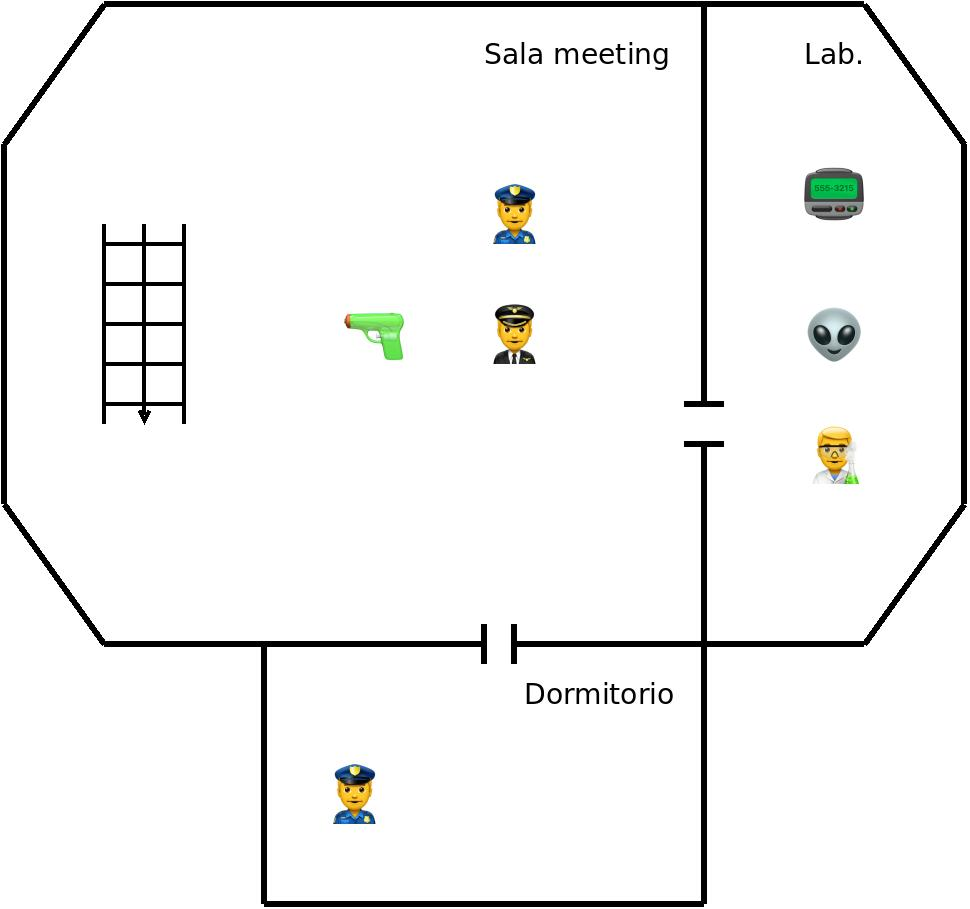
\includegraphics[width=8cm]{map1.jpeg}
			\caption{Mappa primo piano}
			\label{fig:mappa_1}
		\end{figure}
		
		\begin{figure}[!h]
			\centering
			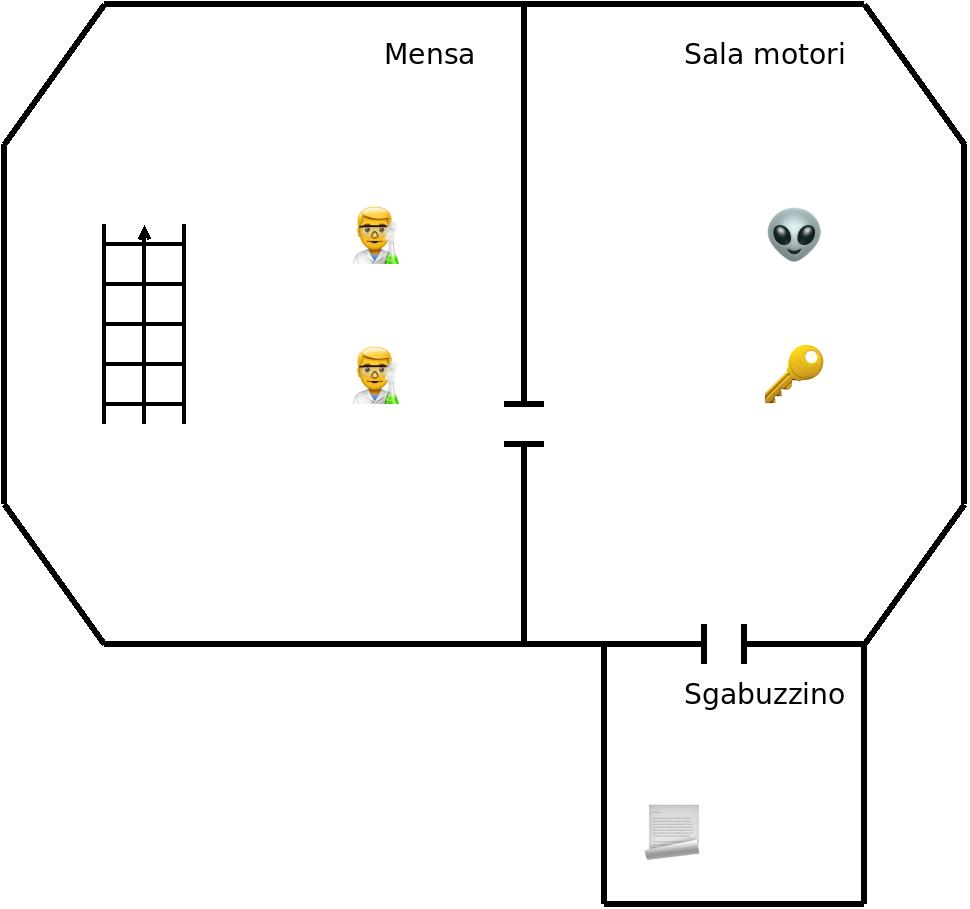
\includegraphics[width=8cm]{map2.jpeg}
			\caption{Mappa secondo piano}
			\label{fig:mappa_2}
		\end{figure}
		

\section{Dettagli implementativi}
	In questa sezione verranno analizzate tutte le tecniche e gli argomenti del corso sfruttati per la realizzazione dell'avventura testuale.
	
	\subsection{Progettazione Object-Oriented}
	
	La progettazione orientata agli oggetti (OOD) è un paradigma di programmazione che utilizza "oggetti" come unità fondamentali per progettare, organizzare e implementare software. Gli oggetti sono istanze di classi, che sono astrazioni che rappresentano concetti, dati e operazioni associati al dominio del problema che si sta affrontando, questa metodologia di progettazione garantisce riutilizzabilità del codice, facilità di manutenzione, chiarezza nel flusso di controllo e scalabilità.\\
	\linebreak
	Nello specifico si sono andate a progettare e realizzare una serie di classi garantendo l'incapsulamento di dati e operazioni, di modo che l'accesso a quest'ultimi sia limitato ai metodi della stessa classe, il che promuove la sicurezza e la modularità del codice.\\
	\linebreak
	Al fine di chiarire la struttura delle classi e delle loro relazioni, abbiamo utilizzato il linguaggio di modellazione UML (Unified Modeling Language) per appresentare in modo visuale la progettazione del software in modo chiaro e conciso.\\
	Il diagramm è presente al seguente link: \href{AGGIUNGERE LINK ALL'IMMAGINE DELL'UML}{diagramma\_uml}  ???????????????????????????

	
	\subsection{File}
	Nel progetto i file sono stati utilizzati per modellare gli elementi narrativi e non dell'avventura, in particolare si hanno a disposizione tre file JSON (JavaScript Object Notation) che vanno a descrivere le stanze, i personaggi e gli oggetti di gioco in modo che le informazioni legate a questi siano facilmente modificabili ed estendibili per migliorare l'avventura, magari aggiungiendo più stanze, modificando i dialoghi dei personaggi e perfino stravolgere la trama di gioco. \\
	\linebreak
	All'avvio del gioco avvene la lettura di questi file per inizializzare tutti i vari oggetti che costituiscono l'avventura, questo avviene utilizzando la libreria \href{https://github.com/FasterXML/jackson}{jackson}, che permette di leggere e utilizzare facilmente i file di tipo JSON, convertendoli in una mappa chiave-valore.
	
	
	\begin{figure}
		\centering
		\subfloat[File delle sanze]{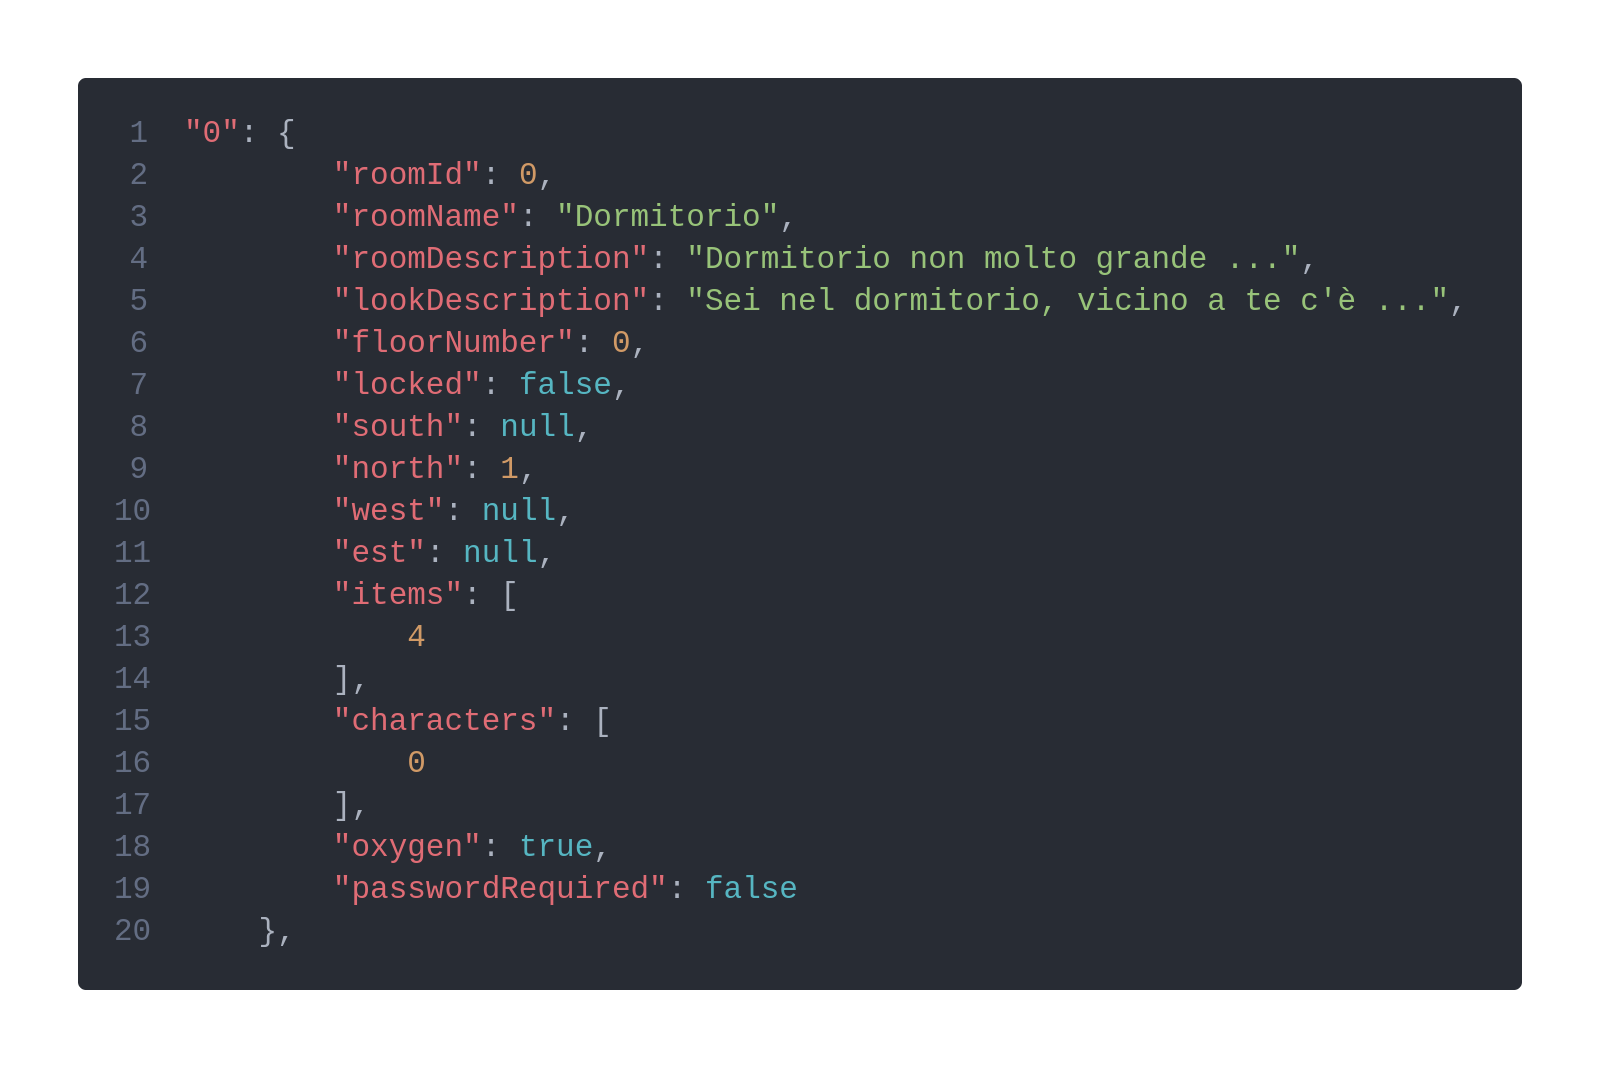
\includegraphics[width=12cm]{code_file1}\label{fig:immagine1}} 
		\\
		\subfloat[File dei personaggi]{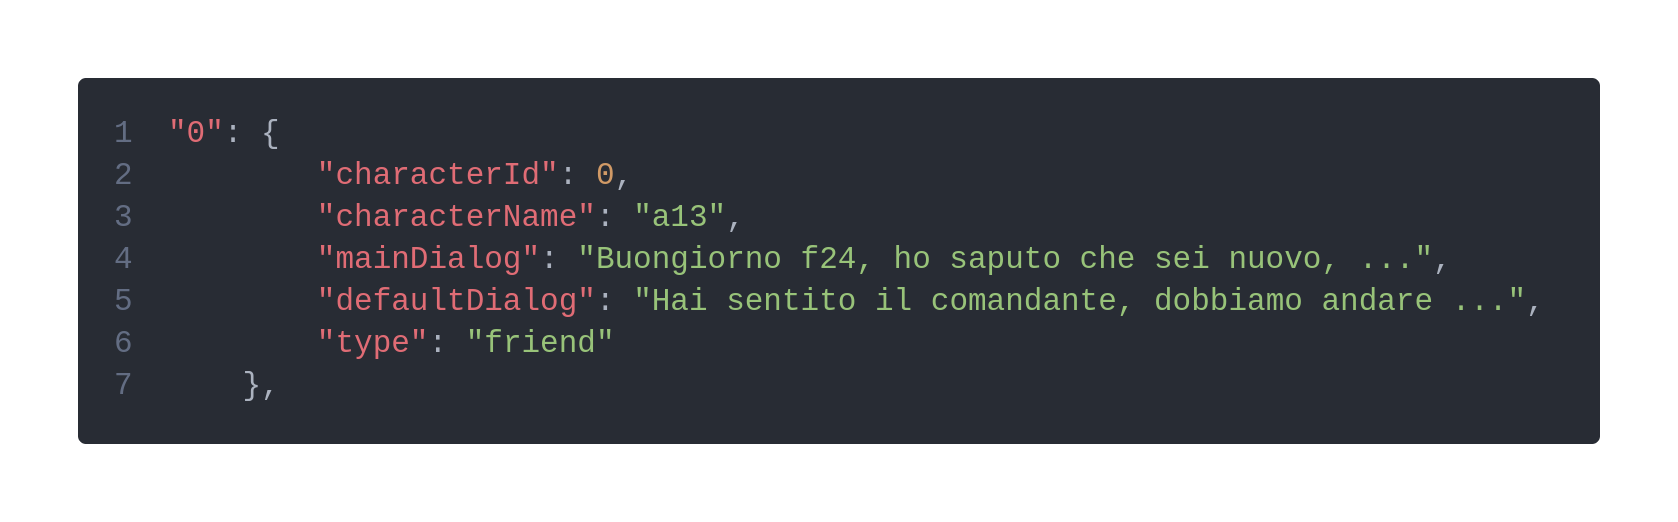
\includegraphics[width=11cm]{code_file2}\label{fig:immagine2}}
		\\
		\subfloat[File degli oggetti]{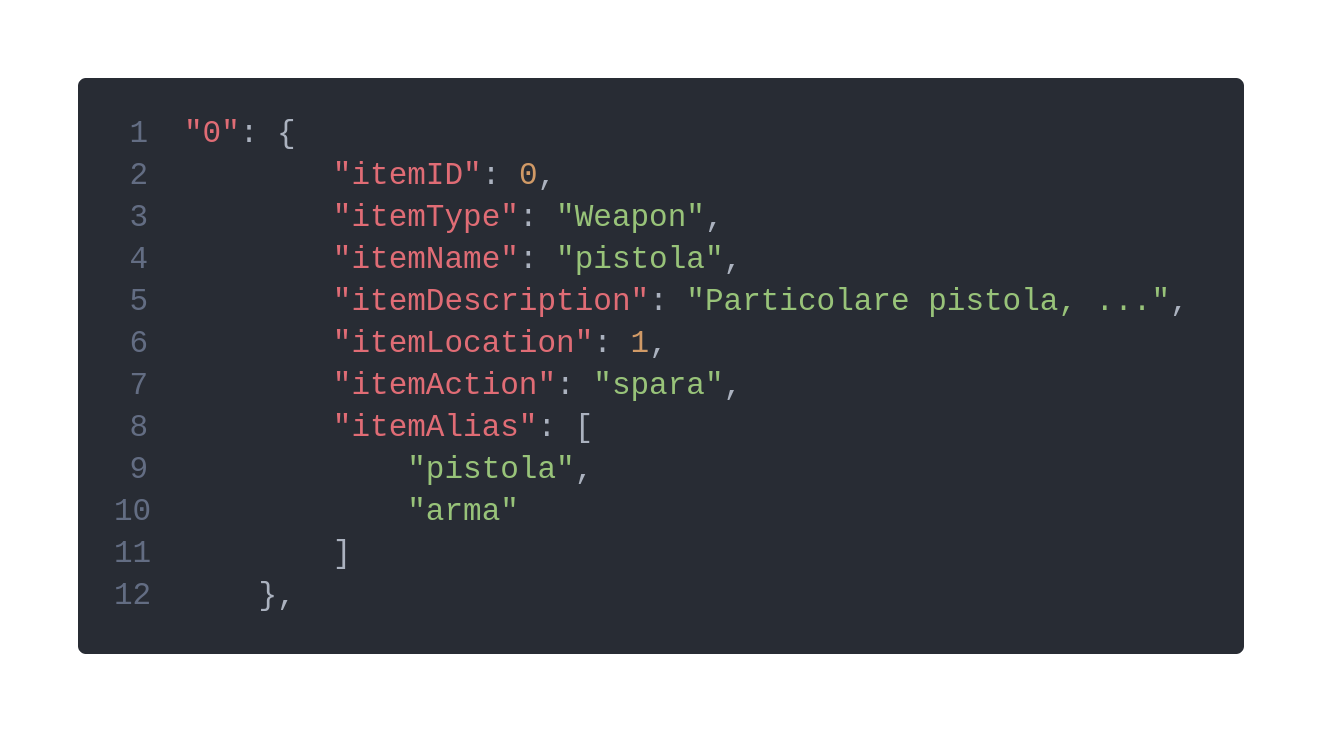
\includegraphics[width=11cm]{code_file3}\label{fig:immagine3}}
		\label{fig:immagini}
	\end{figure}
	
	\subsection{Database}
	
	I salvataggi di gioco sono stati gestiti mediante l'uso della basi di dati, in particolare sono state progettate tre relazioni:
	
	\begin{itemize}
		\item game: memorizza i dati relativi al giocatore, come l'id, la stanza in cui si trova, il numero di nemici eliminati e il timestamp del salvataggio;
		\item inventory: raccoglie tutti gli oggetti recuperati durante l'avventura;
		\item killedCharacter: conserva i dati relativi ai personaggi eliminati nel corso dell'avventura.
	\end{itemize}
	Ogni qual volta che viene salvata la partita, se si esegue il primo salvataggio viene creato il database con le sue relazioni per poi inserirne i relativi dati, altrimenti con il nuovo salvataggio vengono sovrascritti i dati del vecchio.\\
	\linebreak
	Si è pensato di sovrascrivere sempre il salvataggio per motivi di semplicità, ma con la corrente progettazione è possibile modificare quest'aspetto dando la possibilità al giocatore di salvare/caricare più sessioni.\\
	\linebreak
	Esempio:
	\begin{figure}[!h]
		\centering
		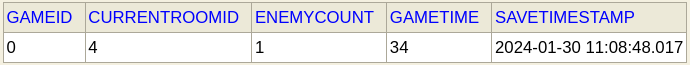
\includegraphics[width=13cm]{db_game.png}
		\caption{Relazione game}
		\label{fig:screen_db1}
	\end{figure}
	\begin{figure}[!h]
		\centering
		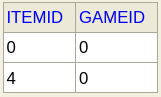
\includegraphics[width=3.5cm]{db_inv.png}
		\caption{Relazione inventory}
		\label{fig:screen_db2}
	\end{figure}
	\begin{figure}[!h]
		\centering
		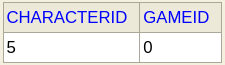
\includegraphics[width=4cm]{db_char.png}
		\caption{Relazione killedCharacter}
		\label{fig:screen_db3}
	\end{figure}
	
	\subsection{Threads}
	\subsection{Api REST}
	\subsection{Java Swing}
	
	\section{Conclusioni}

	\section{Considerazioni finali}
	
	\appendix
	\renewcommand{\thesection}{\Roman{section}}
	\section{Appendice Musica}
	\subsection{Composizione}
	
	Per arricchire l'atmosfera ho incluso nel progetto una mia improvvisazione musicale, cercando di trasmettere un po' quel senso di mistero che avvolge la vicenda di gioco, al fine di far immergere il giocatore ancora meglio nell'avventura.
	
	\subsection{Produzione}
	La parte relativa alla produzione musicale è stata una delle più ardue e al contempo una delle più divertenti, personalmente non mi ero mai cimentato, fino a questo momento, nella produzione di un brano musicale.\\
	\linebreak
	Nello specifico, con la funzione record del pianoforte digitale, ho registrato il barano per poi salvarlo in formato MIDI (Musical Instrument Digital Interface), successivamente ho esportato il file nell'applicazione per Ipad Garagaband, che permette amatorialmente di creare musica, per poi modificare lo strumento di esecuzione, aggiungendo le degli effetti sonori come il wabble ed il riverbero e andando ad esitare la traccia audio, tagliando o registrando nuovamente delle parti, infine ho salvato il tutto sotto froma di WAV (Waveform) per poi imporare il brano nel progetto facendo si che sia riprodotta in loop per tutta la durata del gioco. 
	
	\begin{figure}[!h]
		\centering
		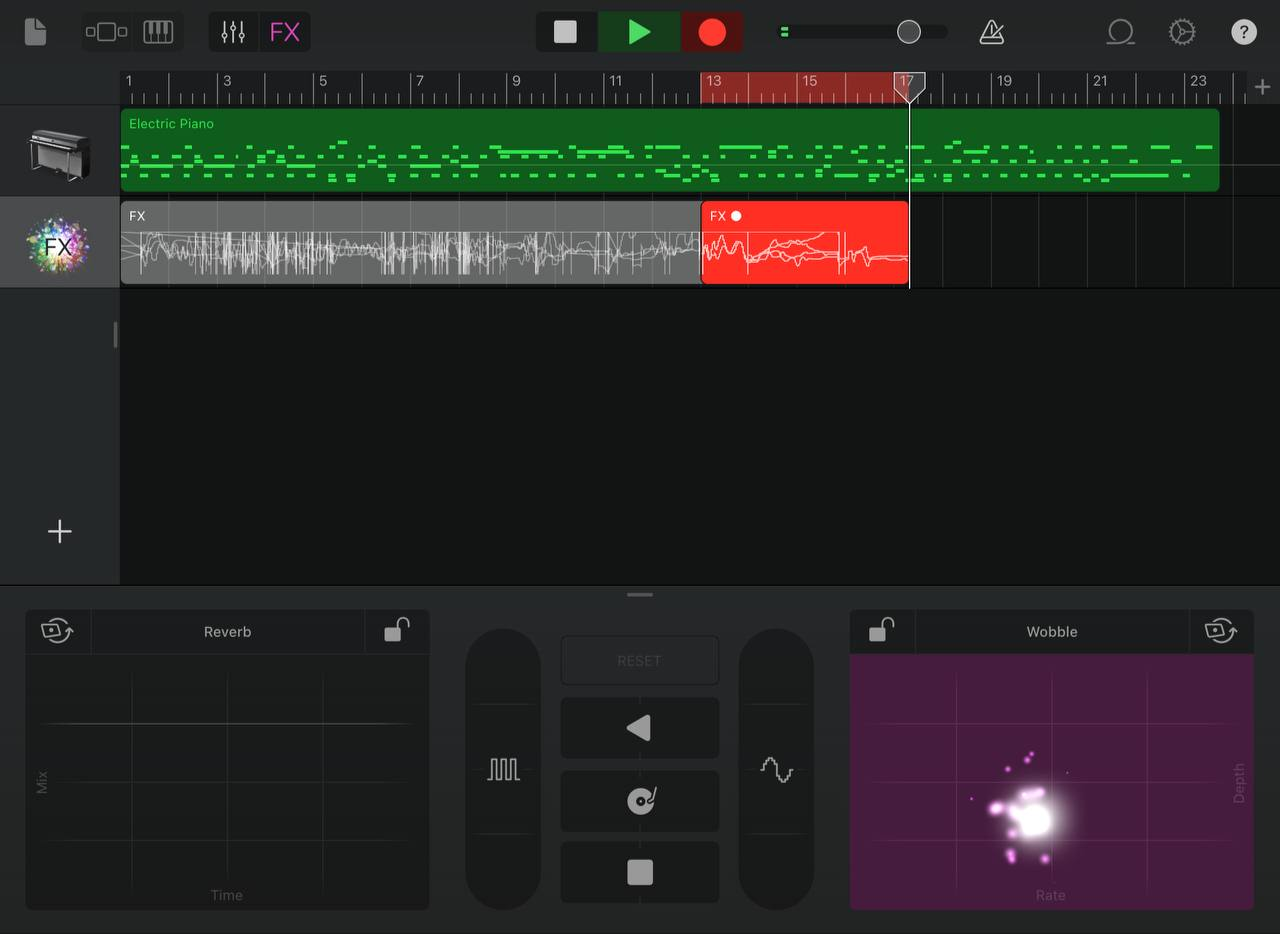
\includegraphics[width=14cm]{garageband.jpg}
		\caption{Screenshot dell'applicazione Garageband}
		\label{fig:musica}
	\end{figure}
	
	
\end{document}